%設定頁面
\documentclass[12pt,a4paper]{article}
\usepackage[margin=1in,a4paper]{geometry}

%設定中文
\usepackage{xeCJK} 
\setCJKmainfont{標楷體} 
\XeTeXlinebreaklocale "zh"   
\XeTeXlinebreakskip = 0pt plus 1pt 

%浮水印
%\usepackage{draftwatermark}
%\SetWatermarkText{\bf NTNU MATH}
%\SetWatermarkScale{0.7}

%圖片
\usepackage{graphicx}
\usepackage{subfigure}

%頁首頁尾
\makeatother
\usepackage{fancyhdr}

%顏色
\usepackage{xcolor}

%設定數學
\usepackage{amsmath, amsthm, amssymb}
\makeatletter

%自定圈圈標號
\usepackage{pstricks,pstricks-add}
\newcommand\textc[1]{{\begin{pspicture*}
(-0.25,-0.2)(0.25,0.3)\rput[c](0,0)
{\large \textcircled{\footnotesize #1}}
\end{pspicture*} }}

%自訂向量符號
\def\leftharpoonfill@{\arrowfill@\leftharpoonup\relbar\relbar}
\def\rightharpoonfill@{\arrowfill@\relbar\relbar\rightharpoonup}
\newcommand\rbjt{\mathpalette{\overarrow@\rightharpoonfill@}}
\newcommand\lbjt{\mathpalette{\overarrow@\leftharpoonfill@}}

%自訂定理
\newtheorem*{thm}{Theorem}
\newtheorem*{lem}{Lemma}
\newtheorem*{de}{Definition}
\newtheorem*{rmk}{Remark}
\newtheorem*{ex}{Example}
\newtheorem*{pf}{Proof}
\newtheorem*{sol}{Solution}

%程式碼
\usepackage{listings}
\usepackage{color}

\definecolor{dkgreen}{rgb}{0,0.6,0}
\definecolor{gray}{rgb}{0.5,0.5,0.5}
\definecolor{mauve}{rgb}{0.58,0,0.82}

\lstset{
  basicstyle={\small \ttfamily},
  frame=tb,
  language=Python,
  aboveskip=3mm,
  belowskip=3mm,
  showstringspaces=false,
  columns=flexible,
  basicstyle={\small\ttfamily},
  numbers=left,
  numbersep = 14pt,
  numberstyle=\tiny\color{gray},
  keywordstyle=\color{blue},
  commentstyle=\color{dkgreen},
  stringstyle=\color{mauve},
  breaklines=true,
  breakatwhitespace=true,
  tabsize=3,
  backgroundcolor=\color{gray!10}
}




%作者
\title{NTNU影像處理HW2}
\author{廖家緯}
\date{2020.3.25}

\begin{document}
\maketitle
%標題、作者、日期
\fontsize{12pt}{20pt}\selectfont
%設定字體大小、間距
\setlength{\baselineskip}{20pt}
%設定行距

\pagestyle{fancy}
\lhead{}
\chead{}
\rhead{}
\lfoot{}
\cfoot{\thepage}
\rfoot{}
\renewcommand{\headrulewidth}{0pt} %上線寬
\renewcommand{\footrulewidth}{0pt} %下線寬
%\renewcommand{\abstractname}{Executive Summary}




%正文開始
\begin{enumerate}
\item[•]{\bf Outline}:
\begin{enumerate}
\item[(A)]Given a grayscale image I,
\begin{enumerate}
\item[\bf Step 1:]
Use the dithering matrix $D_2$ to generate an    
array $D$ of image size by repeating
\vspace*{0.5mm}\\
$D_2$, where
$D_2 = \left[
\begin{array}{cccc}
0 & 128 & 32 & 160\\
192 & 64 & 224 & 96\\
48 & 176 & 16 &144\\
240 & 112 & 208 & 80\\
\end{array}             
\right]$.\vspace*{0.5cm}\\
\item[\bf Step 2:]
Threshold image $I$ by
$I'(i, j) = \begin{cases}
255, & \text{if } I(i,j)>D(i,j)\\
0, & \text{if } I(i,j) \leq D(i,j)
\end{cases}$.
\item[\bf Step 3:]
Show images $I$ and $I'$.\\
\end{enumerate}

\item[(B)]Extend to $n = 4$ gray values
\begin{enumerate}
\item[1.]$\displaystyle \frac{255}{3} = 85$.
\item[2.]$Q(i,j)=
\left[\displaystyle\frac{I(i,j)}{85}\right].$\\
\item[3.]$D_1 = \left[
\begin{array}{cc}
0 & 56\\
84 & 28\\
\end{array}             
\right]
\Longrightarrow D.$
\item[4.]$I'(i, j) = Q(i,j)+\begin{cases}
1, & \text{if } I(i,j)-85Q(i,j)>D(i,j)\\
0, & \text{if } I(i,j)-85Q(i,j)\leq D(i,j)
\end{cases}$.
\item[5.]Scale values of $I'$ so that
its values are in $[0, 255]$ for displaying.
\end{enumerate}
\end{enumerate}

\newpage
\item[•]
{\bf Code(Python):}
\begin{lstlisting}
# coding: utf-8

#引入模組
import numpy as np
import cv2


#(A)讀取灰階影像
I = cv2.imread('Gray.jpg', cv2.IMREAD_GRAYSCALE)
n = np.shape(I)[0]
m = np.shape(I)[1]

#Step1:建構dithering matrix
D2 = np.array([[0, 128, 32, 160], [192, 64, 224, 96], [48, 176, 16, 144], [240, 122, 208, 80]])

#用D2貼滿D
D = np.zeros((n,m), np.int)
for i in range(n):
    for j in range(m):
        D[i, j] = D2[(i%4), (j%4)]
I1 = np.zeros((n,m), np.int)

#Step2:
for i in range(n):
    for j in range(m):
        if I[i, j] > D[i, j]:
            I1[i, j] = 255
        else:
            I1[i ,j] = 0

I1 = np.uint8(I1)

#Step3:
# 顯示原圖I
cv2.imshow('My Image1', I)

# 按下任意鍵則關閉所有視窗
cv2.waitKey(0)
cv2.destroyAllWindows()

# 顯示I1
cv2.imshow('My Image2', I1)

# 按下任意鍵則關閉所有視窗
cv2.waitKey(0)
cv2.destroyAllWindows()
Q = np.zeros((n,m), np.int)


#(B)Extend to n = 4 gray values

#1.
N = np.int(255/3)

#2.
Q = np.zeros((n,m), np.int)

for i in range(n):
    for j in range(m):
        Q[i, j] = I[i, j]/N
        
#3.建構dithering matrix
D1 = np.array([[0, 56], [84, 28]])

#extend to D
D = np.zeros((n,m), np.int)
for i in range(n):
    for j in range(m):
        D[i, j] = D1[(i%2), (j%2)]

#4.
I2 = np.zeros((n,m), np.int)

for i in range(n):
    for j in range(m):
        if I[i, j] - N*Q[i, j] > D[i, j]:
            I2[i, j] = Q[i, j] + 1
        else:
            I2[i, j] = Q[i, j]

#5.
for i in range(n):
    for j in range(m):
        I2[i,j] *= N           
I2 = np.uint8(I2)

# 顯示I2
cv2.imshow('My Image2', I2)

# 按下任意鍵則關閉所有視窗
cv2.waitKey(0)
cv2.destroyAllWindows()


#儲存影像
cv2.imwrite('I.jpg', I)
cv2.imwrite('I1.jpg', I1)
cv2.imwrite('I2.jpg', I2)




\end{lstlisting}

\item[•]
{\bf Result:}
\begin{figure}[h]
\hspace*{10.5em}
\begin{tabular}{c}
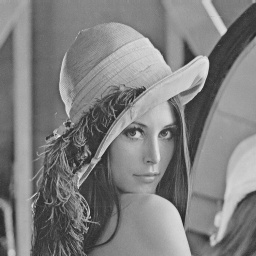
\includegraphics[height=2.4in]{I.jpg}\\
原圖(灰階影像)
\end{tabular}
\end{figure} 

\begin{figure}[h]
\hspace*{3em}
\begin{tabular}{cc}
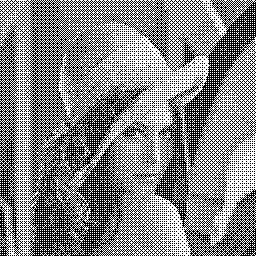
\includegraphics[height=2.4in]{I1.jpg}&
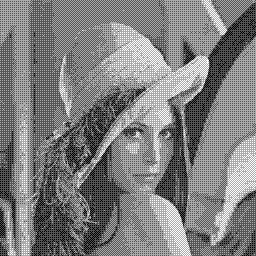
\includegraphics[height=2.4in]{I2.jpg}\\
Threshold image  & $n=4$
\end{tabular}
\end{figure} 

\item[•]
{\bf Experience:}\\
如何將矩陣$D_2$放大至$D$,這裡我嘗試用不同方法,然後Python不像Matlab有許多好用的函式,最後我還是用for迴圈掃過每個元素,搭配mod運算使用。這樣可能提高程式執行的時間複雜度,增加O($n^2$)。而我在寫這支程式的時候是依照老師給的步驟一步步做出來,在我完成之後,了解到這次作業意義:我們將一灰階相片改成用兩個值儲存或著4個值儲存的方法。


\end{enumerate}










\end{document}